\chapter{Expert priors in compartments models: bipolar disorder}
\label{applications-prior_level_vals}

Just as priors in the spline model were influential on the estimates
produced for PMS prevalence in
Chapter~\ref{applications-priors_knots_select}, the priors on the
age-specific rates in a consistent model can be influential on the
estimates.  The situation is more complicated here, however, because
priors on a hazard of one type propagate through to affect the
estimates for all other parameters as well, due to the consistency
enforced by the compartmental model.  In this chapter, we will use the
meta-analysis of bipolar disorder prevalence as an example of the
effects of informative priors on levels of age-specific incidence and
remission hazards.

Bipolar disorder is a mental disorder that causes mood swings
fluctuating between euphoric highs called manic episodes and
depressive lows, interspersed by periods of residual symptoms.  Manic
episodes may last from days to months, causing personal, social and
work-related problems.  Mood swings may occur as infrequently as
yearly or as frequently as several times a day.  Extreme behavior
changes accompany mood changes, and it is not uncommon for sleeping,
eating or activity patterns to change with manic and depressive
episodes.  There is no clear cause for episodes, but life changes,
medications and sleeplessness may trigger manic periods.  
Although residual symptoms can be less severe than manic
and depressive episodes, there is still considerable disability.  While there
is no cure, treatment helps manage mood swings and related
symptoms. \cite{kloos_bipolar_2011, angst_historical_2000}

The modeling of bipolar disorder is based on literature describing it
as a chronic illness with little or no complete remission.  
The terms `residual' and `remission' have very different implications
for the GBD 2010 study.  A residual state involves less severe
symptoms with lesser disability which still contribute to disease
burden.  Remission is equivalent to a cure rather than a temporary
reduction in symptom levels, thus not contributing to burden.  No studies
were found reporting on complete remission from bipolar disorder,
which consistent with the description in the literature that there 
is no cure. \cite{association_diagnostic_2000} 
There is no consistent use of these terms in the bipolar literature, thus
no remission data were included in the modeling.  In this chapter, analysis
only uses data from the GBD 2010 study region of North America, High Income,
shown in Figure~\ref{fig:app-bipolar data}.

    \begin{figure}[h]
        \begin{center}
            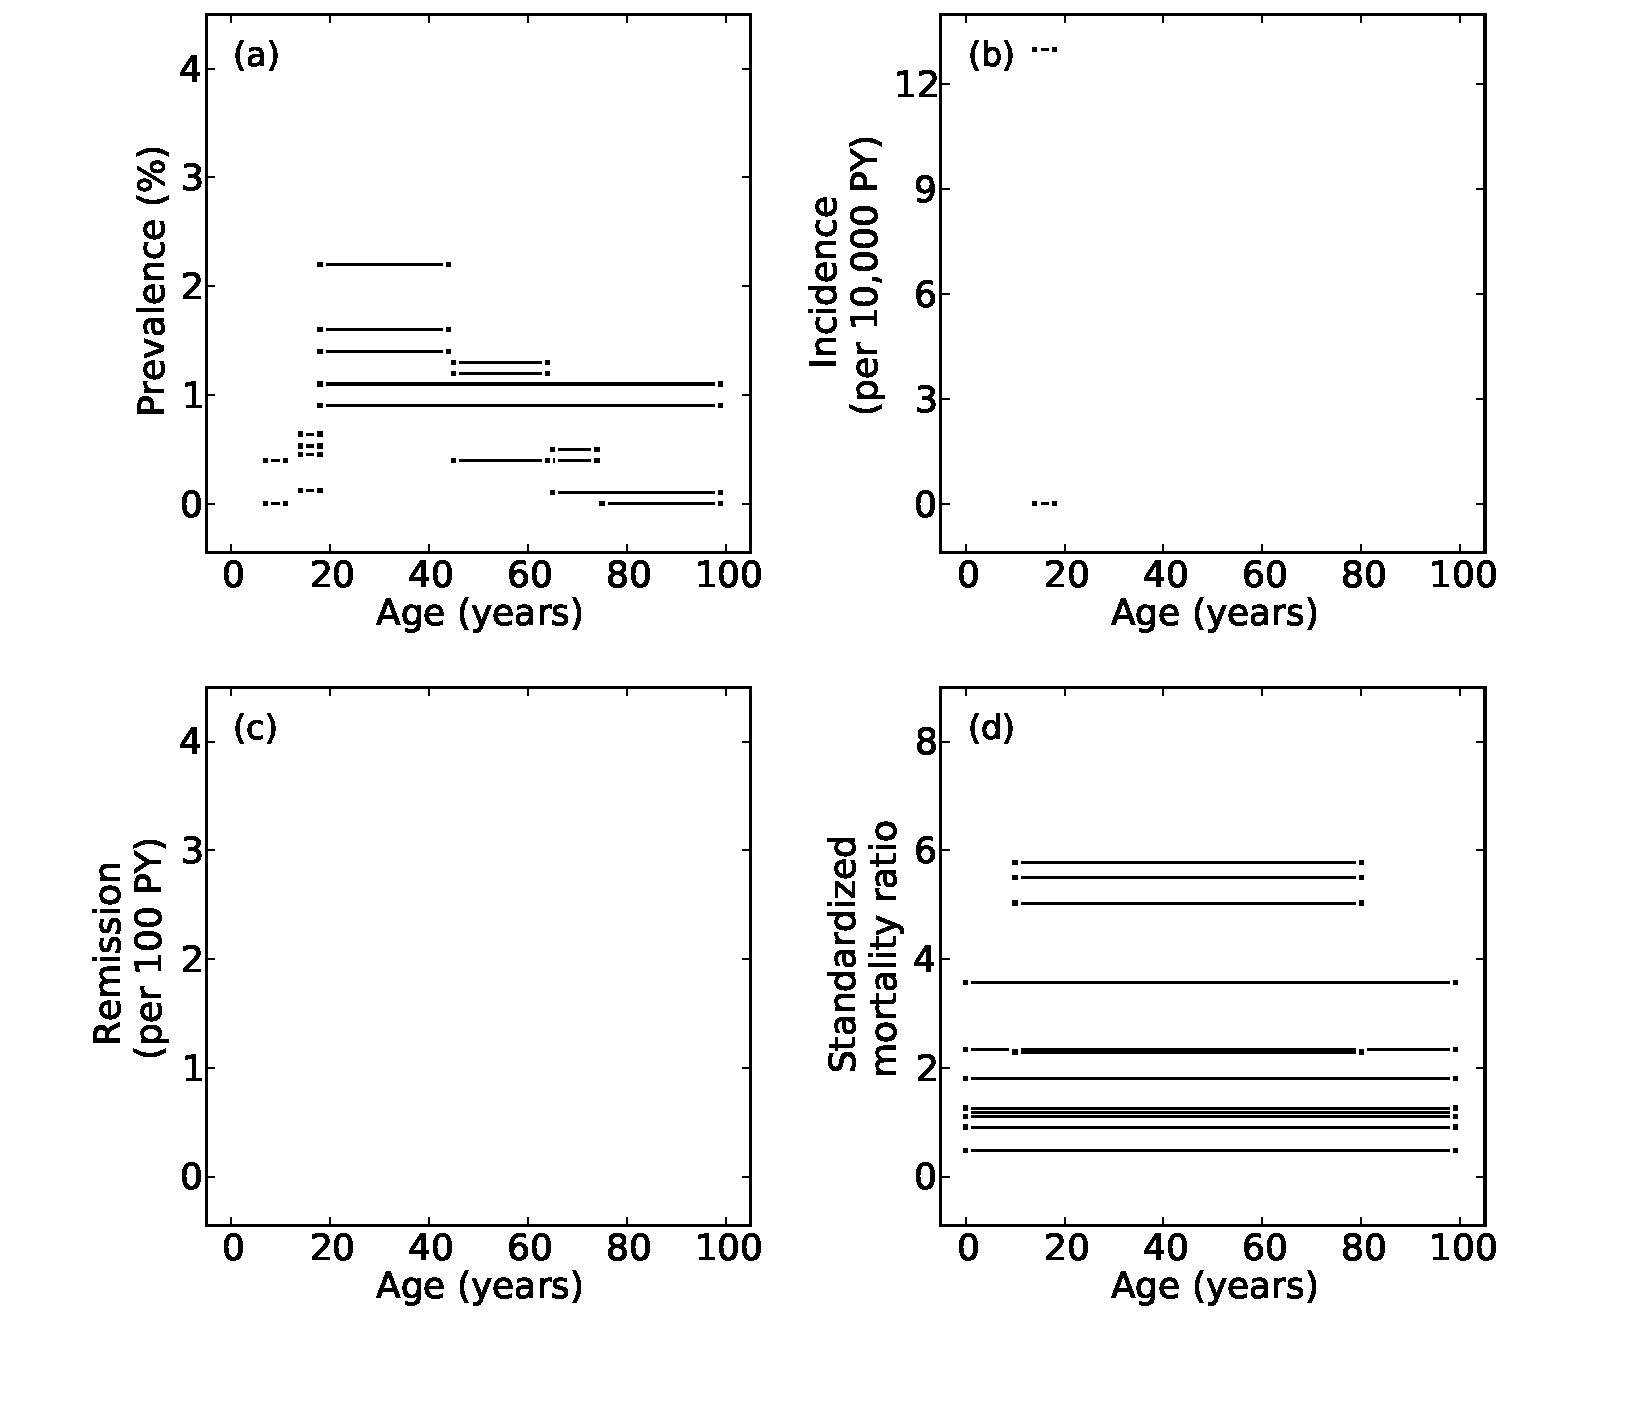
\includegraphics[width=\textwidth]{bipolar-data.pdf}
            \caption{Data included for the modeling of bipolar
              disorder from the GBD 2010 study region of North America,
              high income.}
            \label{fig:app-bipolar data}
        \end{center}
    \end{figure}

%\section{Prevalence and Incidence age of onset}
While there is evidence to suggest that bipolar disorder commonly
starts in the mid-teens or early twenties, there is still disagreement
over a minimum age of onset.  Even though symptoms can be tracked back
to childhood, setting a threshold for diagnosis is difficult given
that current diagnostic criteria are based on the adult presentation of
the disorder.  Literature and expert advice suggest that although
pre-pubertal bipolar disorder is rare, there is a possibility it may
exist. \cite{kloos_bipolar_2011, angst_historical_2000} Therefore the 
estimates presented in Figure~\ref{fig:app-bipolar fit} use a prior 
limiting age of onset to ages 10-80.

    \begin{figure}[h]
        \begin{center}
            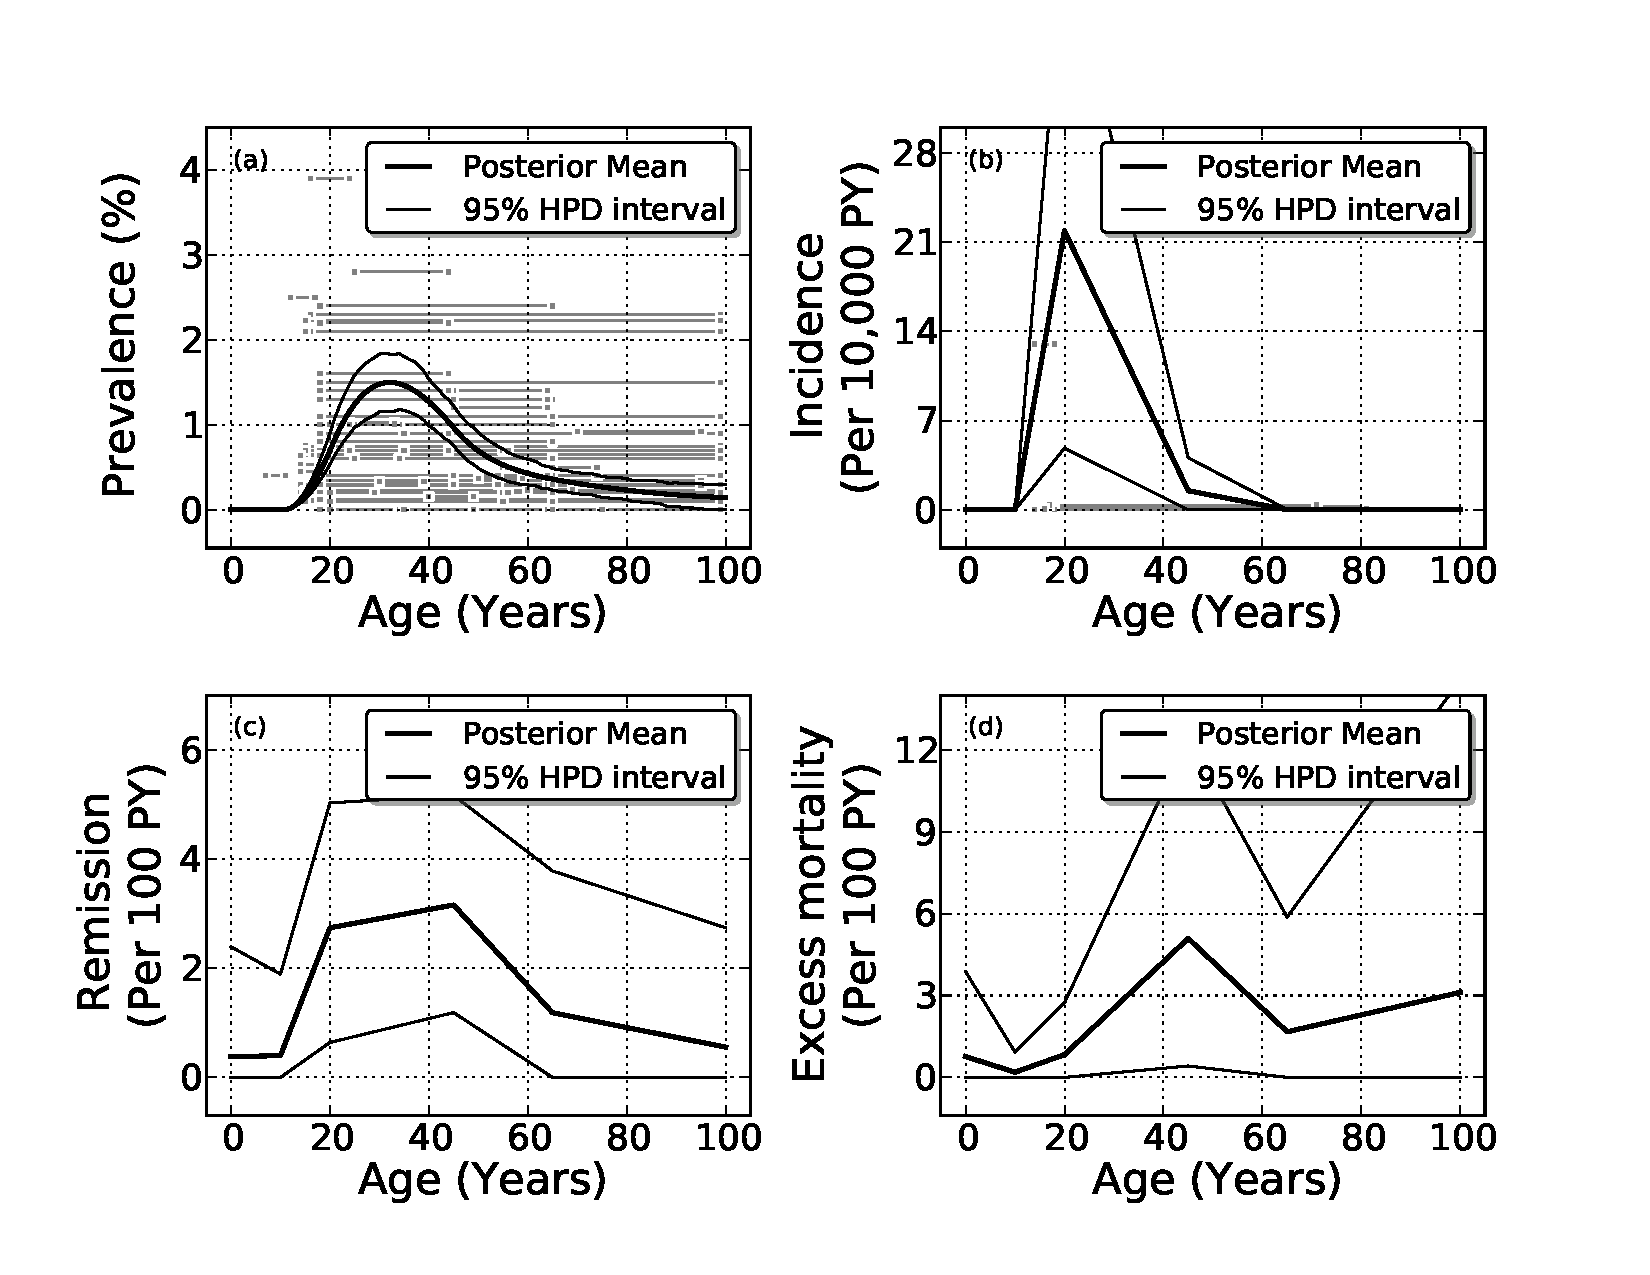
\includegraphics[width=\textwidth]{bipolar-zero_before_ten.pdf}
            \caption{Estimates of bipolar epidemiological parameters for
              males in the GBD 2010 study region of North America, High Income 
              in 1990 using a compartmental model.}
            \label{fig:app-bipolar fit}
        \end{center}
    \end{figure}

While expert priors are useful in guiding the modeling process, they
may have unintended effects as discussed in Chapter~\ref{theory-expert_priors}.  
Choosing to have no restrictions on the
age of onset, the age-specific prevalence differs greatly, as shown in
Figure~\ref{fig:app-bipolar bounds}.

    \begin{figure}[h]
        \begin{center}
            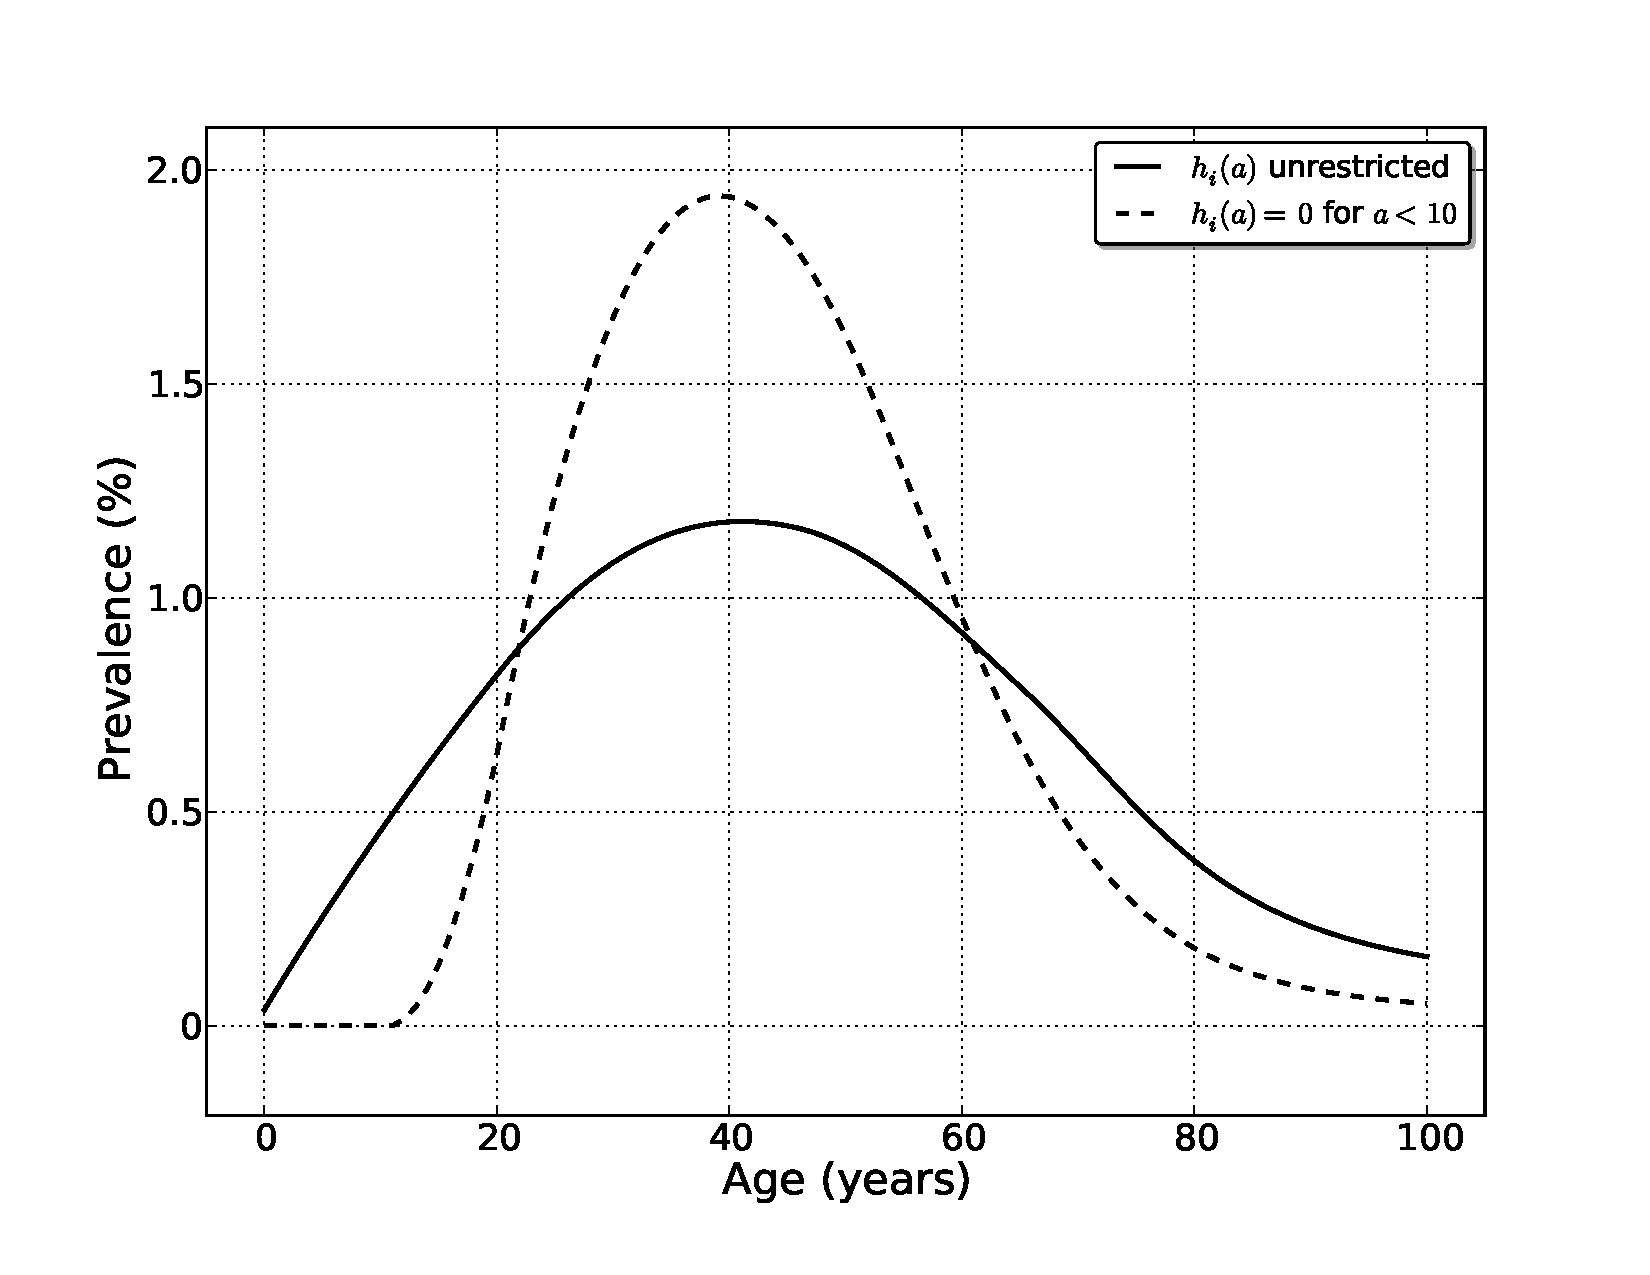
\includegraphics[width=\textwidth]{bipolar-bounds.pdf}
            \caption{Estimates of the prevalence of bipolar disorder
              for males in the GBD 2010 study region of North America, High Income 
              in 1990 using differing priors that limit the age of onset 
              in a compartmental model.}
            \label{fig:app-bipolar bounds}
        \end{center}
    \end{figure}

Like the age of onset, little is known about the upper age limit of
bipolar disorder.  Using expert knowledge to set plausible bounds on the 
level of disease is useful in modeling noisy data--a prior restricting 
the upper age limit of incidence to 65 years led to the most plausible 
fit to the data (Figure~\ref{fig:app-bipolar fit}).  However, changes in the upper age
limit may produce unexpected changes as shown in Figure~\ref{fig:app-bipolar onset}.
The prevalence estimates in Figure~\ref{fig:app-bipolar onset} are about 
the same because there is enough data to inform the model, but incidence, 
remission and excess mortality make subtle changes to account for the prior.

    \begin{figure}[h]
        \begin{center}
            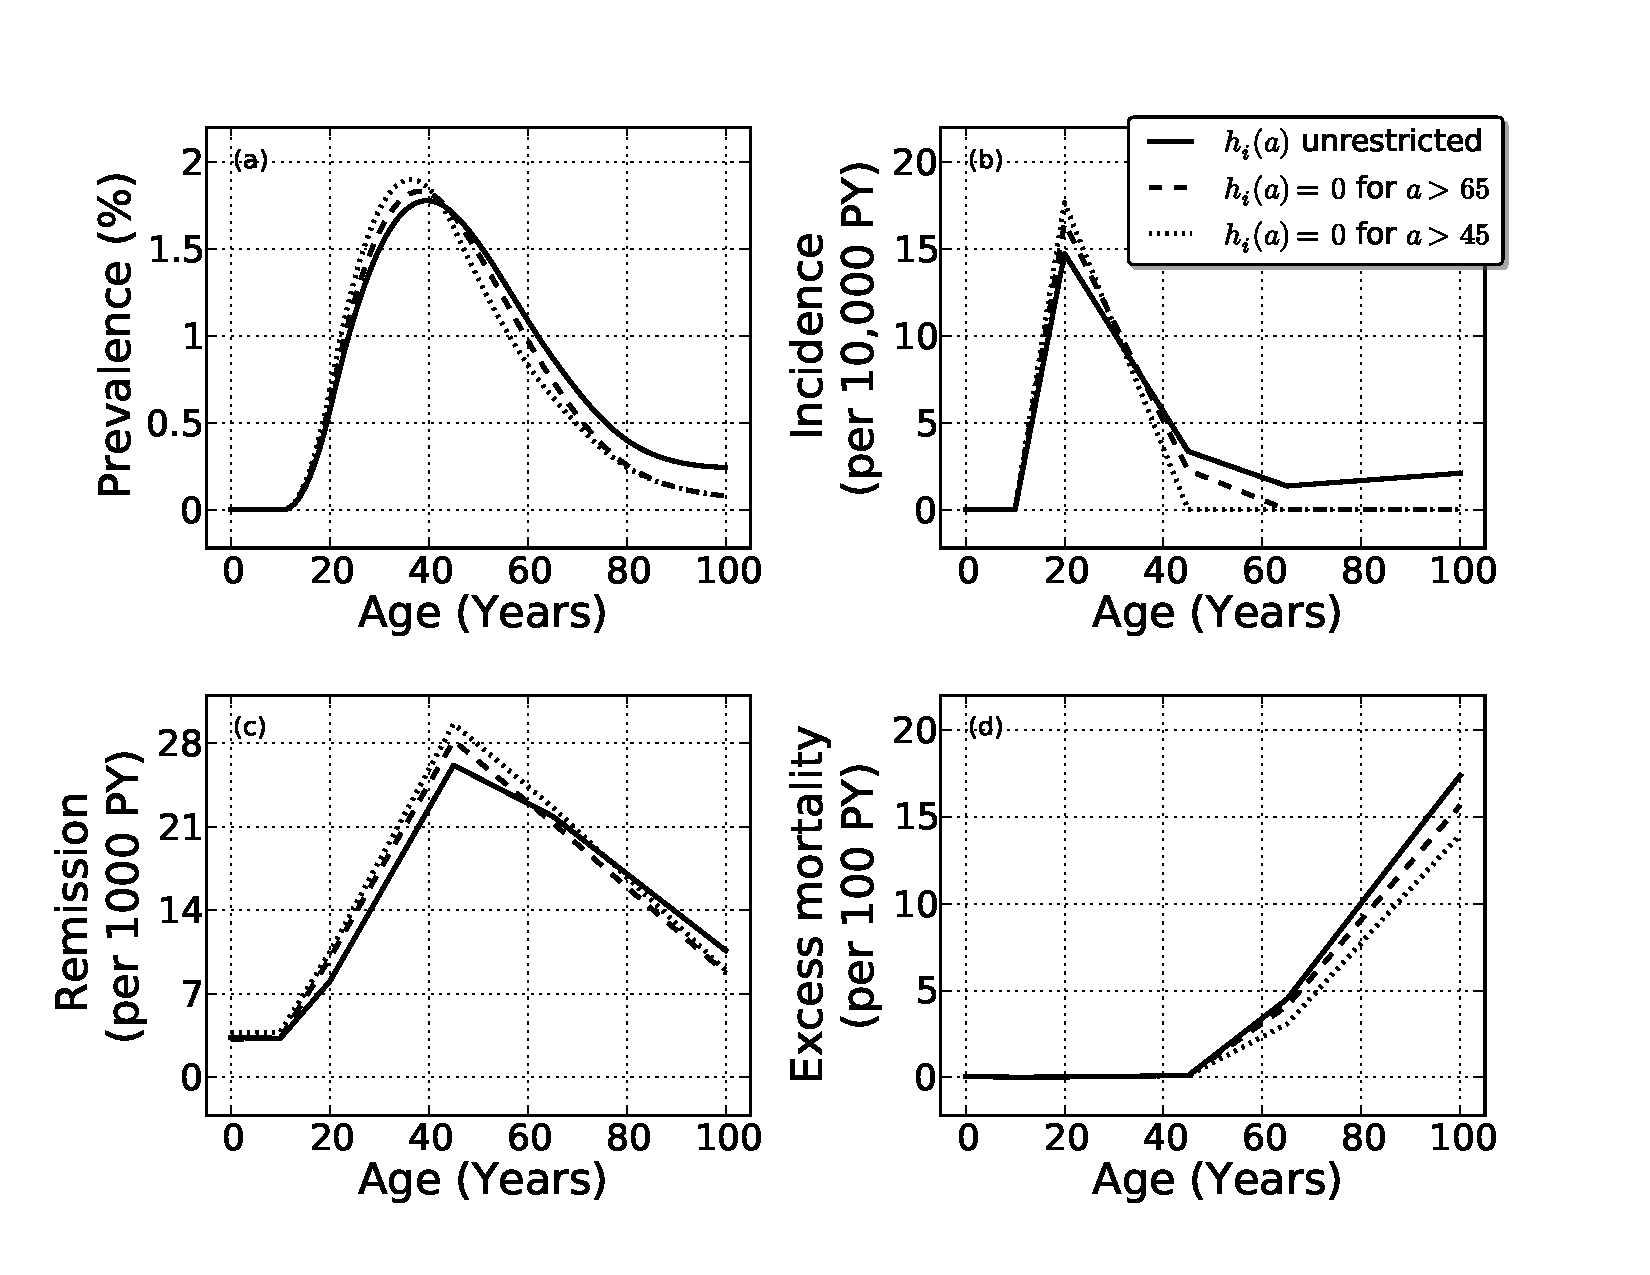
\includegraphics[width=\textwidth]{bipolar-45_65_100.pdf}
            \caption{Estimated prevalence, incidence, remission and
              excess mortality for males with bipolar
              disorder in the GBD 2010 study region of North America, High Income 
              in 1990 using a compartmental model with
              different priors that restrict the upper age limit of
              incidence to 45, 65 or 100.}
            \label{fig:app-bipolar onset}
        \end{center}
    \end{figure}

%\section{Residual v Remission}
Instead, expert guidance set a level prior on the remission rate.  The
compartmental model is sensitive to choice of prior level.  As shown
in the Figure \ref{fig:app-bipolar remission}, choice of prior leads
to large changes in the estimated excess mortality.

    \begin{figure}[h]
        \begin{center}
            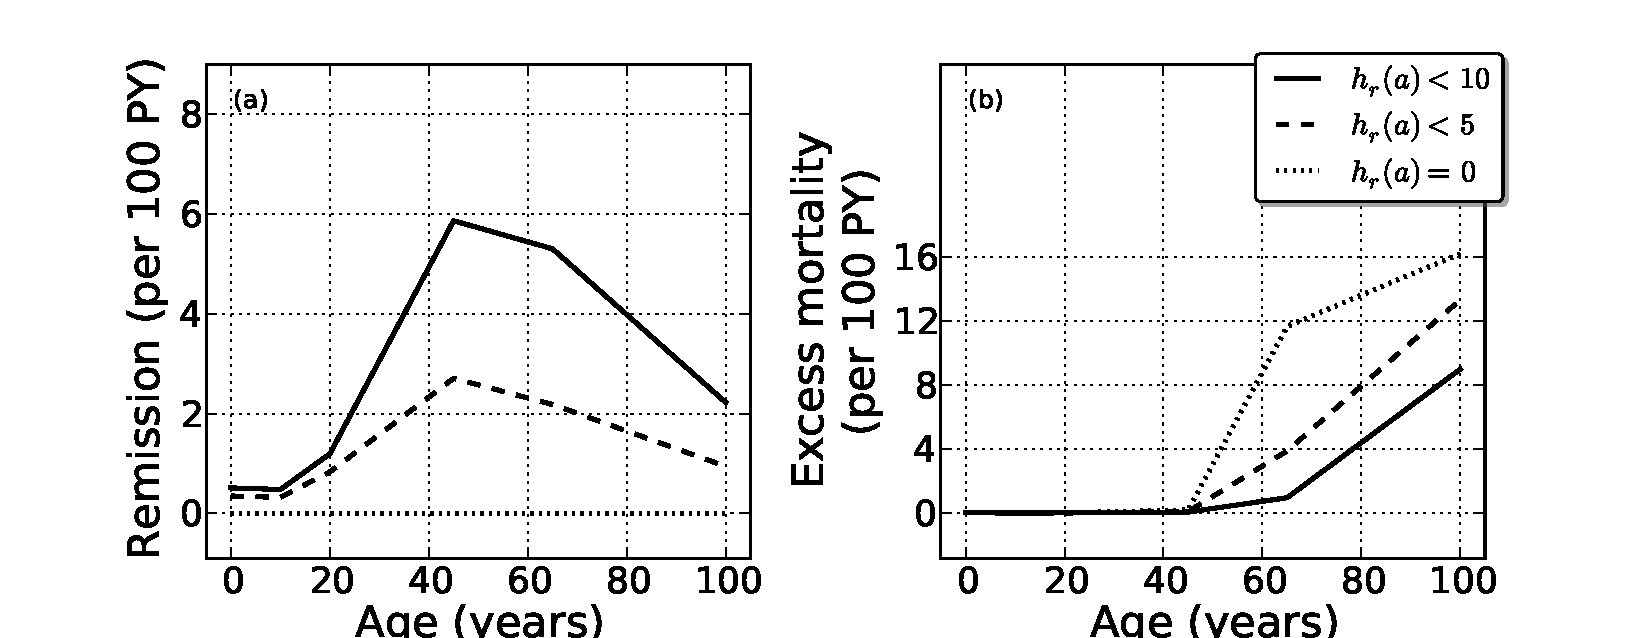
\includegraphics[width=\textwidth]{bipolar-0_5_10.pdf}
            \caption{Remission (panel (a)) and Estimate excess
              mortality (panel (b)) estimates for bipolar disorder in
              males in the GBD 2010 study region of North America, High Income 
              in 1990 in a compartmental model
              with different priors on remission which limit remission
              to 0, 5, 10 per 100 PY.}
            \label{fig:app-bipolar remission}
        \end{center}
    \end{figure}

TK concluding remarks about priors propogating 